\documentclass[a4paper,twoside]{article}
\usepackage{geometry}
\usepackage{amsfonts}
\usepackage{amsthm}
\usepackage{amsmath}
\usepackage{amssymb}
\usepackage[dvips]{graphicx}
\graphicspath{{../figures/}}

\usepackage{mathtools}
\usepackage{float}
\usepackage[section]{placeins}
\usepackage{caption}
\usepackage{subcaption}
\usepackage{notoccite}
\usepackage{tikz}
\usepackage[titletoc]{appendix}
\usepackage{array}
\usepackage{enumitem}
\usepackage{booktabs,siunitx}
\newcommand{\AxisRotator}[1][rotate=0]{\tikz [x=0.25cm,y=0.60cm,line width=.2ex,-stealth,#1] \draw (0,0) arc (-150:150:1 and 1);}

\newtheorem{problem}{Problem}
\newtheorem{theorem}{Theorem}
\newtheorem{proposition}{Proposition}
\newtheorem{corollary}{Corollary}
\newtheorem{lemma}{Lemma}
\newtheorem{definition}{Definition}
\newtheorem{remark}{Remark}

\newtheorem{hd}{HD}

\title{Analysis of the Finite Element Approximability of Three-Dimensional Time-Harmonic Electromagnetic Problems Involving Bianisotropic Materials and 
Metamaterials}
\author{
 Praveen Kalarickel Ramakrishnan\footnote{Department of Electrical, Electtronic, Telecommunications Engineering and Naval Architecture, University of Genoa, Via Opera Pia 11a, I-16145, Genoa, Italy, email:pravin.nitc@gmail.com} \and 
Mario Rene Clemente Vargas\footnote{Department of Electrical, Electtronic, Telecommunications Engineering and Naval Architecture, University of Genoa, Via Opera Pia 11a, I-16145, Genoa, Italy, email:mario.clemente@unige.it} \and 
Mirco Raffetto\footnote{Department of Electrical, Electtronic, Telecommunications Engineering and Naval Architecture, University of Genoa, Via Opera Pia 11a, I-16145, Genoa, Italy, email:raffetto@dibe.unige.it}
}

\begin{document}

\maketitle
\section{Introduction}

\section{Mathematical description of the problem}
In this paper we are interested in electromagnetic problems that involves 
bianisotropic media under time-harmonic excitation, which was studied in 
\cite{kalarickel2020well}.
While the full details of the problem definition and results are available 
in the reference, here we provide a summary of main points in order to 
ease the understanding of the present developments.

The problem is formulated in a domain $\Omega \in \mathbb{R}^3$ 
which has a boundary denoted by $\Gamma$.
The time harmonic sources imply that all the resulting fields 
are in turn time-harmonic and the assumed factor $e^{j\omega t}$ is 
ubiquitous and is suppressed.
The media involved in the problem is linear and time-invariant and 
is considered to be satisfying the following constitutive relations:

    \begin{equation} \label{eq:constitutiveeqn}
      \left\{
        \begin{array}{ll}
          {\bf D} = (1/c_0) \, P \, {\bf E} + L \, {\bf B} 
            & \mbox{ in } \Omega,\\
          {\bf H} = M \, {\bf E} + c_0 \, Q \, {\bf B} 
            & \mbox{ in } \Omega.\\
        \end{array}
      \right.
    \end{equation}

In the above equation, ${\bf E}$, ${\bf B}$, ${\bf D}$ and ${\bf H}$ are 
complex valued functions defined in $\Omega$ and represent, respectively, 
the electric field, magnetic induction, electric displacement, magnetic field 
and $c_0$ is the speed of light in vacuum. 
The space where we will seek ${\bf E}$ and ${\bf H}$ is 
\cite{monkbook} (p. 82; see also p. 69)
%
\begin{equation}
  U=H_{L^2,\Gamma}(\mathrm{curl},\Omega) =
    \{ {\bf v} \in H(\mathrm{curl},\Omega) \; | \;
    {\bf v} \times {\bf n} \in L_t^2(\Gamma) \},
\end{equation}
%
where \cite{monkbook} (p. 48)
%
\begin{equation}
  L_t^2(\Gamma) = \{ {\bf v} \in (L^2(\Gamma))^3 \;|\;
    {\bf v} \cdot {\bf n} = 0 \ \textrm{ almost everywhere on }\Gamma\}.
\end{equation}

Based on Maxwell's equations, boundary conditions and constitutive relations, 
the following variational formulation of the problem can be deduced \cite{bianisotropi_m3as}:
given $\omega>0$, 
  electric and magnetic current densities ${\bf J}_e, {\bf J}_m \in (L^2(\Omega))^3$ 
  and the known term ${\bf f}_R \in L^2_t(\Gamma)$, involved in admittance boundary condition, 
  find ${\bf E} \in U$ such that
  %
  \begin{equation} \label{eq:variationalprob}
    a({\bf E},{\bf v}) = l({\bf v}) \ \ \forall {\bf v} \in U, 
  \end{equation}

\noindent
where
%
\begin{eqnarray} \label{eq:sesquilinear}
  \lefteqn{
    a({\bf u}, {\bf v})
    =
    c_0 
    \big(
      Q \, \mathrm{curl} \, {\bf u}, 
      \mathrm{curl} \, {\bf v}
    \big)_{0,\Omega}
    -
    \frac{\omega^2}{c_0} 
    \big( 
      P \, {\bf u},
      {\bf v}
    \big)_{0,\Omega}
    -
    j \omega
    \big( 
      M \, {\bf u},
      \mathrm{curl} \, {\bf v}
    \big)_{0,\Omega}
  }
  & &
  \nonumber
  \\
  & &
  -
  j \omega
  \big( 
    L \, \mathrm{curl} \, {\bf u},
    {\bf v}
  \big)_{0,\Omega}
  +
  j \omega 
  \big(
    Y \, ({\bf n} \times {\bf u} \times {\bf n}),
    {\bf n} \times {\bf v} \times {\bf n}
  \big)_{0,\Gamma}
  %\ \ {\bf u}, {\bf v} \in U
\end{eqnarray}
%
and
%
\begin{equation} \label{antilinear}
  l({\bf v})
  =
  -
  j \omega 
  \big(
    {\bf J}_e, {\bf v}
  \big)_{0,\Omega}
  -
  c_0
  \big(
    Q \, {\bf J}_m, \mathrm{curl} \, {\bf v}
  \big)_{0,\Omega}
  +
  j \omega 
  \big(
    L \, {\bf J}_m,
    {\bf v}
  \big)_{0,\Omega}
  -
  j \omega 
  \big(
    {\bf f}_R,{\bf n} \times {\bf v} \times {\bf n}
  \big)_{0,\Gamma}.
\end{equation}
%

In \cite{kalarickel2020well} we derived certain sufficient conditions that 
guarantee the well posedness and finite element approximability of the problem.
The developed theory was applied to problems involving rotating axisymmetric objects.
In this paper we apply the theory to a wider range of problems involving bianisotropic media, 
demonstrating the generality of the developments and obtaining interesting new solutions.
In particular we show how the theory can be applied in the presence of metamaterials by 
considering the equivalent media of the type discussed in literature \cite{pendry2016acsphotonics}.

It could be also useful to recall some points on
 how to check for the sufficient conditions that ensure 
the well posedness and finite element approximability of the problem.
In particular it was observed that most of the hypotheses are easily  
verified for important practical problems.
It turns out that the most critical conditions that need to be 
verified are conditions (9) and (10) in \cite{kalarickel2020well}.
These conditions are restated in the following equations. 

\begin{equation}\label{eq:condizione2diteorema2.22delmonk}
  \textrm{for} \ \textrm{every} \ {\bf v} \in U,
  {\bf v} \ne 0, \quad
  \sup_{{\bf u} \in U} \left| a({\bf u}, {\bf v}) \right| > 0,
\end{equation}
%
\begin{equation} \label{eq:infsup}
  \textrm{we} \ \textrm{can} \ \textrm{find} \ \alpha:
  \inf_{ {\bf u} \in U, \ \| {\bf u}\|_U = 1} 
  \sup_{{\bf v} \in U, \ \| {\bf v}\|_U \leq 1} 
    | a({\bf u}, {\bf v}) | \ge \alpha > 0.
\end{equation}
%
As described in \cite{kalarickel2020well}, to satisfy the above conditions,
we need to verify HM9-HM15 in the paper.
Before stating these critical hypotheses a few definitions need to be made.
$\Omega$ is decomposed into $m$ subdomains $\Omega_i$, $i \in I = \{1,2,...m\}$. 
This decomposition can be made such that $I=I_a \cup I_b$, 
where $I_a$ is characterized by subdomains where $L=M=0$. 
Also, an alternative form of constitutive relations given 
in \eqref{eq:constitutiveeqn2} is made use of 
to state some of the hypotheses \cite{noiregolarita}.

\begin{equation} \label{eq:constitutiveeqn2}
  \left\{
    \begin{array}{ll}
      {\bf E} = \kappa \, {\bf D} + \chi \, {\bf B}
        & \mbox{ in } \Omega,\\
      {\bf H} = \gamma \, {\bf D} + \nu \, {\bf B}
        & \mbox{ in } \Omega.\\
    \end{array}
  \right.
\end{equation}

The local continuity of the tensors $P$, $Q$, $L$ and $M$ can be assumed in most 
practical problems and which allows the definiton of the following constants.

\begin{itemize}[leftmargin=*,labelsep=5.8mm] 
  \item 
    $\exists C_L > 0$:
    $| ( L \, \mathrm{curl} \, {\bf u}, {\bf v} )_{0,\Omega} |
    \le 
    C_L \| \mathrm{curl} \, {\bf u} \|_{0,\Omega} \| {\bf v} \|_{0,\Omega}$ 
    for all ${\bf u} \in H(\mathrm{curl}, \Omega)$ and 
    ${\bf v} \in (L^2(\Omega))^3$,
  \item 
    $\exists C_M > 0$:
    $| ( M \, {\bf u}, \mathrm{curl} \, {\bf v} )_{0,\Omega} |
    \le 
    C_M \| {\bf u} \|_{0,\Omega} \| \mathrm{curl} \,{\bf v} \|_{0,\Omega}$ 
    for all ${\bf u} \in (L^2(\Omega))^3$ and 
    ${\bf v} \in H(\mathrm{curl}, \Omega)$.
\end{itemize}
%

Now the important hypotheses are restated here and are renamed as H1-H7.

\begin{description}[leftmargin=32pt,labelsep=7pt]
  \item[H1.]
    $\exists\exists C_{\kappa,d} > 0, \, C_{\nu,d} > 0:
      |determinant\left(\kappa\right)| \ge C_{\kappa,d}, \,
      |determinant\left(\nu\right)| \ge C_{\nu,d}, \, 
      \forall {\bf x} \in \overline{\Omega}_i, \forall i \in I$, 
\end{description}
%
\begin{description}[leftmargin=32pt,labelsep=7pt]
  \item[H2.]
    ${\bf l}_{1,3}^T \, \kappa^{-1} \, {\bf l}_{1,3} \ne 0, \
    {\bf l}_{1,3}^T \, \nu^{-1} \, {\bf l}_{1,3} \ne 0 \
    \forall {\bf l}_{1,3} \in \mathbb{R}^3, {\bf l}_{1,3} \ne 0, \
    \forall {\bf x} \in \overline{\Omega}_i, \, \forall i \in I_a$,
\end{description}
%
\begin{description}[leftmargin=38pt,labelsep=7pt]
  \item[H3.]
    $\exists \exists C_{\kappa,r} > 0, \ C_{\nu,r} > 0: \ 
      |{\bf l}_{1,3,n}^T \, \kappa^{-1} \, {\bf l}_{1,3,n}| \ge C_{\kappa,r}, \
      |{\bf l}_{1,3,n}^T \, \nu^{-1} \, {\bf l}_{1,3,n}| \ge C_{\nu,r}
      \ \forall {\bf l}_{1,3,n} \in \mathbb{R}^3: \| {\bf l}_{1,3,n} \|_2 = 1, \
      \forall {\bf x} \in \overline{\Omega}_i, \, \forall i \in I_b$,
\end{description}
%
\begin{description}[leftmargin=32pt,labelsep=7pt]
  \item[H4.]
    $\exists \exists C_{\kappa,s} > 0, C_{\nu,s} > 0$:
    %
    \begin{equation}
      \big( \sum_{i, j = 1}^3 |\kappa_{ij}| \big) - 
        \min_{i=1,2,3} |\kappa_{ii}| \le C_{\kappa,s}
      \quad \forall {\bf x} \in \overline{\Omega}_k, \, \forall k \in I_b,
    \end{equation}
    %
    \begin{equation}
      \big( \sum_{i, j = 1}^3 |\nu_{ij}| \big) - 
        \min_{i=1,2,3} |\nu_{ii}| \le C_{\nu,s}
      \quad \forall {\bf x} \in \overline{\Omega}_k, \, \forall k \in I_b,
    \end{equation}
    %
    and $\kappa$, $\chi$, $\gamma$ and $\nu$ satisfy
    %
    \begin{equation} \label{condizionesubianisotropixalgogenerale}
      \frac{4 \,
            \Big( \big( \sum_{i, j = 1}^3 |\gamma_{ij}| \big) - 
                  \min_{i=1,2,3} |\gamma_{ii}| \Big)
            \,
            \Big( \big( \sum_{i, j = 1}^3 |\chi_{ij}| \big) - 
                  \min_{i=1,2,3} |\chi_{ii}| \Big)
           }{
        \big( 
          - C_{\kappa,s} + 
          \sqrt{ C_{\kappa,s}^2 + 4 \, C_{\kappa,d} \, C_{\kappa,r}} 
        \big) \, 
        \big( 
          - C_{\nu,s} + 
          \sqrt{ C_{\nu,s}^2 + 4 \, C_{\nu,d} \, C_{\nu,r}} 
        \big)} 
      < 1
    \end{equation}
    %
    $\forall {\bf x} \in \overline{\Omega}_k, \, \forall k \in I_b$.
\end{description}
%

\begin{description}
  \item[H5.]
    We can find $C_{PS} > 0$ such that 
    $|(P {\bf u}, {\bf u})_{0,\Omega}| 
    \ge 
    C_{PS} \| {\bf u} \|_{0,\Omega}^2$ 
    for all ${\bf u} \in (L^2(\Omega))^3$.
\end{description}
%
\begin{description}
  \item[H6.]
    We can find $C_{QS} > 0$ such that 
    $|(Q \mathrm{curl} \, {\bf u}, \mathrm{curl} \, {\bf u})_{0,\Omega}| 
    \ge 
    C_{QS} \| \mathrm{curl} \, {\bf u} \|_{0,\Omega}^2$ 
    for all ${\bf u} \in H(\mathrm{curl}, \Omega)$.
\end{description}
% 

\begin{description}
  \item[H7.]
    $C_{PS}$, $C_{QS}$, $C_L$ and $C_M$ (i.e., all media involved) 
    are such that  $C_{QS} - \frac{C_L C_M}{C_{PS}} > 0$.
\end{description}
%

The section ``some hints to apply the developed theory'' 
of \cite{kalarickel2020well}, provided the guidance to use 
the theory that was developed.
Lemma 1 of the above paper provides a procedure to check 
conditions H5 and H6 and thus estimate the constants 
$C_{PS}$ and $C_{QS}$ which may in turn be used to check H7. 
Let $P$ be decomposed as $P=P_s - jP_{ss}$, and if 
$P_{ss}$ is uniformly positive definite in some region $\Omega_{el}$
and $P_s$ is uniformly positive definite in the complementary region 
$\Omega \setminus \Omega_{el}$, then H5 can be shown to be true 
in the following way.
We can define $C_1 >0$ and $C_2 >0$ as follows.

\begin{equation} \label{eq:c1_constant}
    \int_{\Omega_{el}}{\bf u}^*P_{ss}{\bf u} \geq C_1 \int_{\Omega{el}}|{\bf u}|^2 = C_1 ||{\bf u}||^2_{0, \Omega_{el}} \hbox{   } \forall {\bf u} \in (L^2(\Omega))^3,
\end{equation}

\begin{equation} \label{eq:c2_constant}
    \left|\int_{\Omega \setminus \Omega_{el}} {\bf u}^*P_s{\bf u}\right| \geq C_2||{\bf u}||^2_{0,\Omega \setminus \Omega_{el}}.
\end{equation}

The continuity of $P_s$ in $\Omega_{el}$ allows the definition of $C_3 > 0$ such that 
  \begin{equation} \label{eq:c3_constant}
    \left| \int_{\Omega_{el}} {\bf u}^* P_s {\bf u} \right| \le 
      C_3 \|{\bf u}\|^2_{0,\Omega_{el}}.
  \end{equation}

If $\Omega_{el}=\Omega$, then we can take $C_{PS} = C_1$, if 
$\Omega_{el} = \emptyset$ then $C_{PS} = C_2$ and in other cases

  \begin{equation} \label{eq:cps_metamaterial}
    C_{PS} = 
      \frac{1}{\sqrt{2}} 
      \min 
      \left( 
        \sqrt{(1-\alpha)} C_2, \sqrt{C_1^2+(1-\frac{1}{\alpha}) C_3^2}
      \right),
  \end{equation}
  %
  where $\alpha$ is such that 
  $1 > \alpha > \frac{C_3^2}{C_1^2+C_3^2} > 0$.

Similar considerations can help to estimate $C_{QS}$ as well.

The values obtained above may not the best possible ones than can 
be estimated and the 
condition in H7 can be made less restrictive 
if the estimates of $C_{PS}$ and $C_{QS}$ can be higher.
For example, whenever $P_s$ is uniformly definite 
in $\Omega$, we have $C_4 >0$ such that

\begin{equation} \label{eq:c4_constant}
  \left| \int_{\Omega} {\bf u}^*P_s{\bf u} \right| 
  \geq 
  C_4||{\bf u}||^2_{0,\Omega}.
\end{equation}

In this case, the best value for $C_{PS}$ would be the 
larger among the one in \eqref{eq:cps_metamaterial} and $C_4$.
Based on the definitions, the constants $C_L$ and $C_M$ can
be  estimated and the validity of H7 can be checked.

\begin{equation} \label{equationnumber27}
  C_L = 
    \max_{i \in I_b} 
    \sup_{{\bf x} \in \Omega_i} \sqrt{\lambda_{max}(L^* L)} 
\end{equation}
%
and 
%
\begin{equation} \label{equationnumber28}
  C_M = 
    \max_{i \in I_b} 
    \sup_{{\bf x} \in \Omega_i} \sqrt{\lambda_{max}(M^* M)},
\end{equation}

As for the constants involved in H1-H4,  the following considerations
can be helpful.

\begin{equation} \label{equationnumber29}
  C_{\kappa, d} = 
    \min_{i \in I_b} \inf_{{\bf x} \in \Omega_i} 
    |determinant(\kappa)|,
\end{equation}
%
\begin{equation} \label{equationnumber30}
  C_{\nu, d} = 
    \min_{i \in I_b} \inf_{{\bf x} \in \Omega_i} 
    |determinant(\nu)|,
\end{equation}
%
\begin{equation} \label{equationnumber31}
  C_{\kappa,s} = 
    \max_{i \in I_b} \sup_{{\bf x} \in \Omega_i} 
      \left((\sum_{i,j=1}^3|\kappa_{ij}|)-\mathrm{min}_{i=1,2,3}|\kappa_{ii}| \right),
\end{equation}
%
\begin{equation} \label{equationnumber32}
  C_{\nu,s} = 
    \max_{i \in I_b} \sup_{{\bf x} \in \Omega_i} 
    \left((\sum_{i,j=1}^3|\nu_{ij}|)-\mathrm{min}_{i=1,2,3}|\nu_{ii}| \right).
\end{equation}
%

As for $C_{\kappa, r}$ and $C_{\nu, r}$ the following consideration
might be helpful.
By definition
%
\begin{equation} \label{equationnumber33}
  C_{\kappa, r} = 
    \min_{i \in I_b} \inf_{{\bf x} \in \Omega_i} \quad
    \min_{{\bf l}_{1,3,n} \in \mathbb{R}^3: \| {\bf l}_{1,3,n} \|_2 = 1} 
    \sqrt{\left(
            {\bf l}_{1,3,n}^T \kappa_{is} {\bf l}_{1,3,n}
          \right)^2 
          + 
          \left(
            {\bf l}_{1,3,n}^T \kappa_{iss} {\bf l}_{1,3,n}
          \right)^2},
\end{equation}
%
\begin{equation} \label{equationnumber34}
  C_{\nu, r} = 
    \min_{i \in I_b} \inf_{{\bf x} \in \Omega_i} \quad
    \min_{{\bf l}_{1,3,n} \in \mathbb{R}^3: \| {\bf l}_{1,3,n} \|_2 = 1} 
    \sqrt{\left(
            {\bf l}_{1,3,n}^T \nu_{is} {\bf l}_{1,3,n}
          \right)^2 
          + 
          \left(
            {\bf l}_{1,3,n}^T \nu_{iss} {\bf l}_{1,3,n}
          \right)^2},
\end{equation}
%
where $\kappa_{is}$ and $\kappa_{iss}$ are the symmetric matrices 
obtained by the usual decomposition of $\kappa^{-1}$ and similarly 
$\nu_{is}$ and $\nu_{iss}$ are those corresponding to $\nu^{-1}$. 
If both the symmetric matrices involved in the above expressions are 
semi-definite, then we can deduce the following lower bounds:
%
\begin{equation} \label{equationnumber35}
  C_{\kappa, r} = 
    \min_{i \in I_b} \inf_{{\bf x} \in \Omega_i}
    \sqrt{ \left( \lambda_{min}(\kappa_{is}) \right)^2 
           + 
           \left( \lambda_{min}(\kappa_{iss}) \right)^2},
\end{equation}
%
\begin{equation} \label{equationnumber36}
  C_{\nu, r} = 
    \min_{i \in I_b} \inf_{{\bf x} \in \Omega_i}
    \sqrt{ \left( \lambda_{min}(\nu_{is}) \right)^2 
           + 
           \left( \lambda_{min}(\nu_{iss}) \right)^2}.
\end{equation}
%

If we also define
%
\begin{equation} \label{equationnumber37}
  C_{\chi,s} = 
    \max_{i \in I_b} \sup_{{\bf x} \in \Omega_i} 
      \left((\sum_{i,j=1}^3|\chi_{ij}|)-\mathrm{min}_{i=1,2,3}|\chi_{ii}| \right),
\end{equation}
%
\begin{equation} \label{equationnumber38}
  C_{\gamma,s} = 
    \max_{i \in I_b} \sup_{{\bf x} \in \Omega_i} 
    \left((\sum_{i,j=1}^3|\gamma_{ij}|)-\mathrm{min}_{i=1,2,3}|\gamma_{ii}| \right),
\end{equation}
%
the sufficient condition for the regularity used for proving 
uniqueness can be expressed as
%
\begin{equation} \label{equationnumber39}
  K_{u} = 
  \frac{4 C_{\chi,s} C_{\gamma,s}}{
  \left( -C_{\kappa,s} + \sqrt{C_{\kappa,s}^2+4C_{\kappa,d}C_{\kappa,r}} \right)
  \left( -C_{\nu,s} + \sqrt{C_{\nu,s}^2+4C_{\nu,d}C_{\nu,r}} \right)} < 1.
\end{equation}
%

\section{Results and discussion}  
In this section we apply the theory developed in \cite{kalarickel2020well} to 
several different class of problems which could not be managed with the 
previous theory like the one in \cite{bianisotropi_m3as}.
The conditions are established on the parameters of such problems, 
under which the well posedness and finite element 
approximability  can be guaranteed.
Under such condition, the numerical solutions for the fields are 
computed for the first time.
The details of our finite element simulator is the same as that 
described in Section 5 of \cite{kalarickel2020well}.
%In particular let us first consider the class of problems involving materials described in Kraft et al. \cite{pendry2016acsphotonics}.

\subsubsection{Plasmonic gratings considered in \cite{pendry2016acsphotonics} behaving as bianisotropic metamaterial}
In  \cite{pendry2016acsphotonics}, Kraft et. al consider a plasmonic grating 
which exhibits bianisotropy at visible wavelength.
Here we consider scattering problems involving an equivalent medium 
that can be characterized by the constitutive matrices of the same form 
given in the paper.
The region occupied by the scatterer may be denoted as $\Omega_s \subset \Omega$. 
We start with the form of the normalized constitutive relation as found in 
\cite{chen2005retrieval} and \cite{li2009determination}, 
and obtain the $P$, $Q$, $L$, $M$ matrices \cite{noiregolarita}.
The final form given below is obtained by considering 
non magnetic material with 
$\mu_r=1$ and with an isotropic complex relative permittivity $\varepsilon_r$. 
The magnetoelectric coupling parameter is denoted $\zeta_0$. 

\begin{equation}  \label{constitutive_kraft_P}
P = c_0 \varepsilon_0 
\begin{bmatrix}
\varepsilon_r & 0 & 0 \\
0 &  \varepsilon_r & 0 \\
0 & 0 & \varepsilon_r-\zeta_0^2
\end{bmatrix} 
\end{equation}

\begin{equation} \label{constitutive_kraft_Q}
Q = \frac{1}{c_0\mu_0}I
\end{equation}

\begin{equation} \label{constitutive_kraft_LM}
L = M^T = \frac{j\zeta_0}{\mu_0 c_0}
\begin{bmatrix}
0 & 0 & 0 \\
0 & 0 & 0 \\
0 &  1  & 0
\end{bmatrix} 
\end{equation}
 
The complementary region $\Omega \setminus \Omega_s$ is 
occupied by the empty space, which,  in our notation, is characterized by 
 $P=c_0\varepsilon_0I_3$, $Q=\frac{1}{c_0\mu_0}I_3$, $L=M=0$.

The bianisotropic medium is lossy with the imaginary part $Im(\varepsilon_r) < 0$, 
where as $\zeta_0$ is assumed real here to avoid some longer calculation. 
Now Lemma 1 of \cite{kalarickel2020well} can be applied to verify hypothesis H5.
Inside $\Omega_s$, $P$ can be decomposed as $P= P_s -j P_{ss}$ with
\begin{equation}
P_s = \frac{P+P^*}{2} =  c_0\varepsilon_0
\begin{bmatrix}
Re(\varepsilon_r) & 0 & 0 \\
0 & Re(\varepsilon_r) & 0 \\
0 & 0 & Re(\varepsilon_r) - \zeta_0^2 \\
\end{bmatrix},
\end{equation}
and  $P_{ss} = \frac{P^*-P}{2j} =  -c_0\varepsilon_0 Im(\varepsilon_r) I_3$.
Hence we have $\Omega_{el} = \Omega_s$, the lossy region 
where $P_{ss}$ is uniformly positive definite 
and the complementary region with free space where $P_s$ 
is uniformly positive definite.
This means that the conditions of relevant Lemma are satisfied and 
as a result H5 is valid.

From the definitions
$C_1=c_0\varepsilon_0 |Im(\varepsilon_r)|$, 
$C_2 = c_0\varepsilon_0$ and 
$C_3 = c_0\varepsilon_0 \max(|Re(\varepsilon_r) -\zeta_0^2|, |Re(\varepsilon_r)|)$.
To find the minimum of the two expressions in \eqref{eq:cps_metamaterial},
we note that, in the valid range, the value of the 
first expression decreases monotonically with  $\alpha$ where as
that of the second expression increases with it. 
The highest estimate for $C_{PS}$  is obtained when the two expressions 
have the same value.
The value of $\alpha$ at which this happens can be evaluated by 
equating the two expressions and finding the positive 
root of the resulting quadratic equation.
This value of $\alpha$, denoted as $\alpha_{opt}$ is given by 
\eqref{eq:alpha_opt}.

\begin{equation}  \label{eq:alpha_opt}
\alpha_{opt} = \frac{C_2^2-C_1^2-C_3^2 + \sqrt{(C_2^2-C_1^2-C_3^2)^2+4C_2^2C_3^2}}{2C_2^2}
\end{equation}

Thus we may simply write 
\begin{equation} \label{eq:cps_metamaterial_optimal}
C_{PS} = \sqrt{\frac{1-\alpha_{opt}}{2}}c_0\varepsilon_0.
\end{equation}
As mentioned before, this does not mean that a better value of $C_{PS}$ 
cannot be found.
For example, if $Re(\varepsilon_r) -\frac{\zeta_0^2}{\mu_r} > 0$, 
then $P_s$ is uniformly positive definite in $\Omega$ and we can find 
another candidate for $C_{PS}$, namely $C_4 = c_0\varepsilon_0\min(1, |Re(\varepsilon_r-)\zeta_0^2|$.
In particular, when  $Re(\varepsilon_r) - \zeta_0^2 > 1$, $C_4 = c_0\varepsilon_0$ is always going to give a value for $C_{PS}$ which is higher than that obtained from the Lemma.

The generality of out theory be clearly demonstrated by showing its 
applicability to bianisotropic metamaterials. 
Hence in the rest of the subsection the discussion  focuses on 
the cases with $\varepsilon_r < 0$.
For this case,$C_3 = c_0\varepsilon_0 |Re(\varepsilon_r) -\zeta_0^2|$ , and we can directly use the value of $C_{PS}$ in \eqref{eq:cps_metamaterial_optimal}.
Since the material is assumed to be non magnetic the direct application of definition 
gives $C_{QS} = \frac{1}{c_0\mu_0}$.
Likewise, the continuity constants $C_L = C_M = \frac{|\zeta_0|}{c_0\mu_0}$.
Then the inequality in H7 becomes $C_{QS} -\frac{C_L C_M}{C_{PS}} = \frac{1}{c_0\mu_0}(1 -\frac{\zeta_0^2\sqrt{2}}{\sqrt{1-\alpha_{opt}}}) > 0$, 
which gives \eqref{eq:inequality_zeta0}.

\begin{equation} \label{eq:inequality_zeta0}
|\zeta_0| < \left(\frac{1 - \alpha_{opt}}{2}\right)^{1/4}.
\end{equation}

Since the right hand side of \eqref{eq:inequality_zeta0} also depends on 
$\zeta_0$ due to the presence of $C_3$ in the expression for $\alpha_{opt}$,
we do not have a closed form expression on the limit on $\zeta_0$ 
below which H7 is satisfied.
However a graphical analysis can be done for estimating such a limit 
on $|\zeta_0|$, as shown in 
Figure \ref{fi:critical_zeta_vs_epsilonr_inf_sup}.
The value of $Re(\varepsilon_r)$ is varied in the range $(-1.0,-5.0)$ 
whereas $Im(\varepsilon_r)$ assumes values in the range $(-0.1,-0.5)$.
It can be observed that for a fixed value of $Im(\varepsilon_r)$, 
the range of $\zeta_0$ over which H7 is valid steadily decreases as 
$|Re(\varepsilon_r)|$ increases. 
As for the dependence on $Im(\varepsilon_r)$, the corresponding range
increases when medium becomes more lossy due to higher $|Im(\varepsilon_r)|$,
as expected.

\begin{figure}[H]
\centering
\begin{subfigure}[b]{0.49\textwidth}
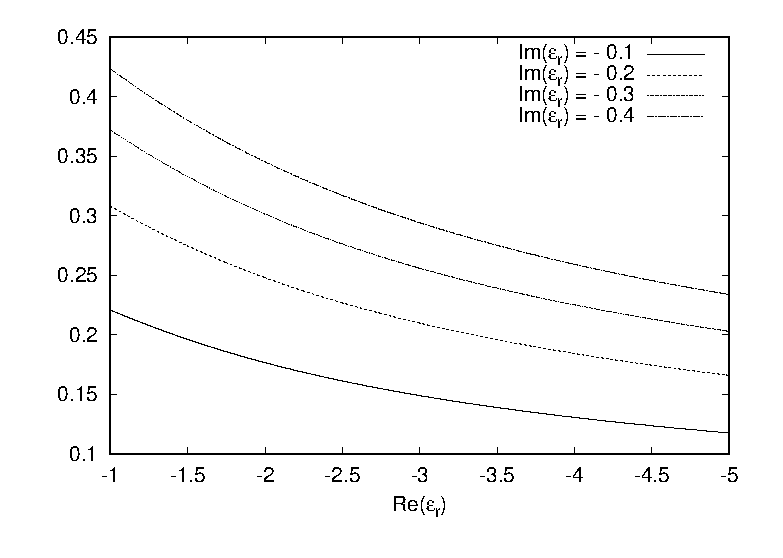
\includegraphics[width=\textwidth]{critical_zeta_vs_real_epsilon_pendry_inf_sup.eps}
\end{subfigure}
%
\begin{subfigure}[b]{0.49\textwidth}
\centering
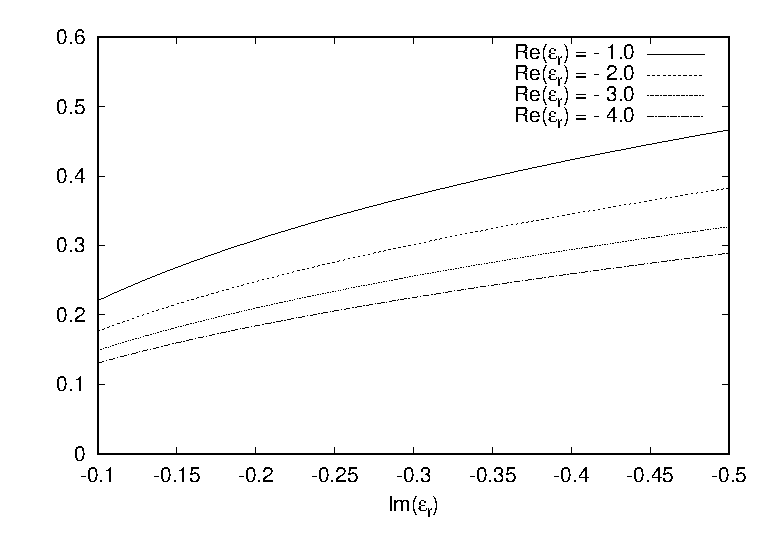
\includegraphics[width=\textwidth]{critical_zeta_vs_imag_epsilon_pendry_inf_sup.eps}
\end{subfigure}
\caption{The magnitude of $|\zeta_0|$ below which the condition \ref{eq:infsup} is satisfied as a function of $Re(\varepsilon_r)$ or $Im(\varepsilon_r)$ for media in Kraft et al.
The plot is for real $\zeta_0$ negative values of  $Re(\varepsilon_r)$ or $Im(\varepsilon_r)$ and the material is taken to be non magnetic.}
\label{fi:critical_zeta_vs_epsilonr_inf_sup}
\end{figure}

We consider the alternative form of constitutive relations , 
which for the medium inside $\Omega_s$ becomes as
in equations \eqref{constitutive_kraft_kappa} to \eqref{constitutive_kraft_chi_gamma}, 
for examining the validity of H1-H4 \cite{noiregolarita}.

\begin{equation} \label{constitutive_kraft_kappa}
\kappa = \frac{1}{\varepsilon_0\varepsilon_r}
\begin{bmatrix}
1 & 0 & 0 \\
0 & 1 & 0 \\
0 & 0 & \frac{\varepsilon_r}{\varepsilon_r-\zeta_0^2}
\end{bmatrix}
\end{equation}

\begin{equation} \label{constitutive_kraft_nu}
\nu = \frac{1}{\mu_0}
\begin{bmatrix}
1 & 0 & 0 \\
0 & \frac{\varepsilon_r}{\varepsilon_r - \zeta_0^2} & 0 \\
0 & 0 & 1
\end{bmatrix}
\end{equation}

\begin{equation} \label{constitutive_kraft_chi_gamma}
\gamma = -\chi^T = \frac{j\zeta_0c_0}{\varepsilon_r-\zeta_0^2}
\begin{bmatrix}
0 & 0 & 0 \\
0 & 0 & 1 \\
0 & 0 & 0
\end{bmatrix}
\end{equation}

Since H1-H4 needs to hold only locally, and they are trivially 
valid in the empty space outside the bianisotropic media, 
we have to just analyze them inside $\Omega_s$ occupied by the bianisotropic medium.
These constants can be evaluated directly from the definitions. 
The determinants of $\kappa$ and $\nu$ are, respectively, 
$\frac{1}{(\varepsilon_0 \varepsilon_r)^3(1-\frac{\zeta_0^2}{\varepsilon_r})}$ and
$\frac{1}{(\mu_0)^3(1-\frac{\zeta_0^2}{\varepsilon_r})}$  which immediately give the values of  $C_{\kappa,d}$ and $C_{\nu,d}$.

\begin{equation}
C_{\kappa,d} =  \frac{1}{|\varepsilon_0^3\varepsilon_r^3(1 - \frac{\zeta_0^2}{\varepsilon_r})|}, 
\end{equation}

\begin{equation}
C_{\nu,d} =  \frac{1}{|\mu_0^3(1 - \frac{\zeta_0^2}{\varepsilon_r})|}.
\end{equation}

The inverses of the diagonal matrices $\kappa$ and $\nu$ are just the 
diagonal matrices with the reciprocal entries.
Applying equations \eqref{equationnumber35} and \eqref{equationnumber36} gives the values of $C_{\kappa,r}$ and $C_{\nu,r}$.

\begin{equation}
C_{\kappa,r} =  |\varepsilon_0\varepsilon_r (1 - \frac{\zeta_0^2}{\varepsilon_r})|,
\end{equation}

\begin{equation}
C_{\nu,r} =  |\mu_0 (1 - \frac{\zeta_0^2}{\varepsilon_r})|. 
\end{equation}

Using equations \eqref{equationnumber35} and \eqref{equationnumber36} we get the $C_{\kappa,s}$ and $C_{\nu,s}$.

\begin{equation}
C_{\kappa,s} =  \frac{1}{\varepsilon_0} \max(\frac{2}{|\varepsilon_r|}, \frac{1}{|\varepsilon_r|}(1 + \frac{1}{|1 - \frac{\zeta_0^2}{\varepsilon_r}|})),
\end{equation}

\begin{equation}
C_{\nu,s} = \frac{1}{\mu_0} \max(2, (1 + \frac{1}{|1 - \frac{\zeta_0^2}{\varepsilon_r}|})),
\end{equation}

Since we are interested in the case when $Re(\varepsilon_r) < 0$ and real $\zeta_0$, 
 we see that $|1 - \frac{\zeta_0^2}{\varepsilon_r}| > 1$,   and the maximum reduces to 
the values in \eqref{eq:cks_pendry} and \eqref{eq:cnus_pendry}.

\begin{equation} \label{eq:cks_pendry}
C_{\kappa,s} =  \frac{2}{|\varepsilon_0\varepsilon_r|},
\end{equation}

\begin{equation} \label{eq:cnus_pendry}
C_{\nu,s} = \frac{2}{\mu_0}. 
\end{equation}

Using equations \eqref{equationnumber37} and \eqref{equationnumber38} 
we can easily evaluate $C_{\gamma,s}$ and $C_{\chi,s}$. 

\begin{equation}
C_{\gamma,s} =  C_{\chi,s} = |\frac{\zeta_0c_0}{\varepsilon_r - \zeta_0^2}|. 
\end{equation}

Using these constants, the value of $K_u$  can be calculated using equation \eqref{equationnumber39}.
The critical value of $|\zeta_0|$ below which the condition in H4 is satisfied is plotted in Figure \ref{fi:critical_zeta_vs_epsilonr_uniqueness}, 
with respect to either $Re(\varepsilon_r)$ or $Im(\varepsilon_r)$.
The results show that the range of $\zeta_0$ for which H4 holds true increases with the increase in $|Re(\varepsilon_r)|$, 
while it is practically independent of $Im(\varepsilon_r)$.

\begin{figure}[H]
\centering
\begin{subfigure}[b]{0.49\textwidth}
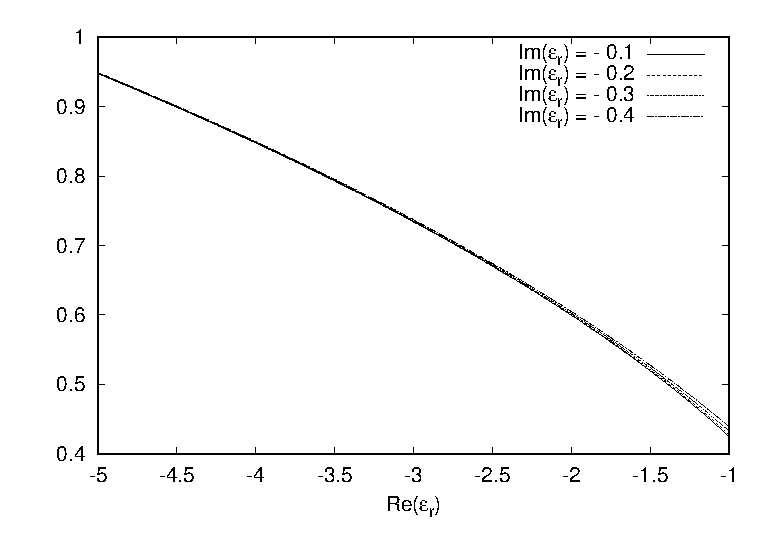
\includegraphics[width=\textwidth]{critical_zeta_vs_real_epsilon_pendry_uniqueness.eps}
\end{subfigure}
%
\begin{subfigure}[b]{0.49\textwidth}
\centering
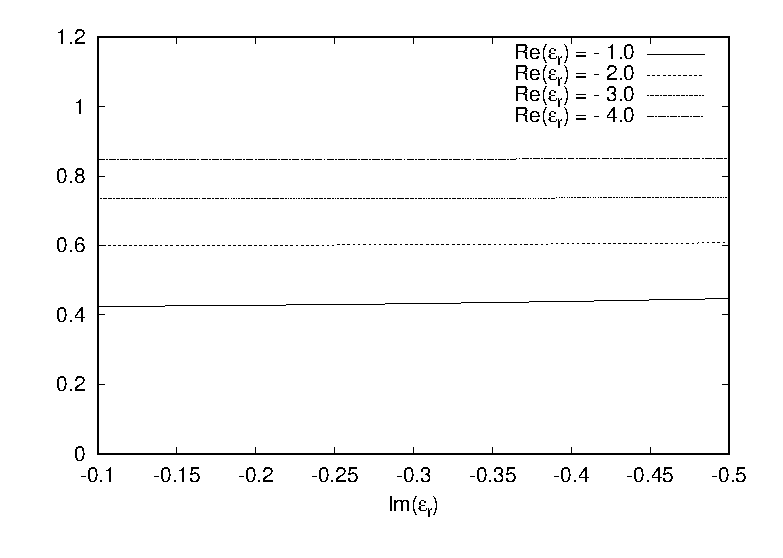
\includegraphics[width=\textwidth]{critical_zeta_vs_imag_epsilon_pendry_uniqueness.eps}
\end{subfigure}
\caption{The magnitude of $\zeta_0$ below which the condition \ref{eq:condizione2diteorema2.22delmonk} is satisfied as a function of $Re(\varepsilon_r)$ or $Im(\varepsilon_r)$ for media in Kraft et al.
The plot is for real $\zeta_0$ and the material is taken to be non magnetic.}
\label{fi:critical_zeta_vs_epsilonr_uniqueness}
\end{figure}

Let us try to understand the implications of the theory by applying it to 
the numerical solution of a specific problem involving the medium of interest.
We consider the region with the scatterer $\Omega_{s}$ to be a cube filled 
with homogeneous bianisotropic media.
The surrounding region is filled with empty space and the overall domain 
of numerical investigation, $\Omega$, is of cubic shape as well, and is 
concentric to $\Omega_{s}$.
In the following $\Omega$ is characterized by sides of length 2 $\mu m$ 
and $\Omega_s$ by those of 0.8 $\mu m$.
The axes are taken along the sides of the cubes and the excitation is 
with a plane wave incident along the x axis, with electric field polarized along 
z axis, having a magnitude of 1 $V/m$ and wavelength of 1 $\mu m$.

Inside $\Omega_s$, the medium is characterized by $\varepsilon_r = -1 - j0.4$, 
$\mu_r = 1$ and $\zeta_0 = -0.41$. 
This value is such that the hypotheses required for well posedness and 
finite element approximability are satisfied.
In fact, for the $\varepsilon_r$ considered, condition \ref{eq:condizione2diteorema2.22delmonk} 
is valid for $|\zeta_0| < 0.4235$ and condition \ref{eq:infsup} is valid for 
$|\zeta_0| < 0.4393$.

The solutions are obtained with a first order edge element based Galerkin 
finite element method. The boundary condition is enforced with $Y$ equal to 
the admittance of vacuum and with an inhomogeneous term ${\bf f}_R$, 
taking into account the incident field. 

The domain is discretized uniformly using tetrahedral meshes.
The meshing is done by first dividing the domain into small identical cubes,
each of which is in turn divided into six tetrahedra.
The parameter $h$ denotes the maximum diameter of all the elements of the 
mesh \cite{handbook} (p. 131), and in this case it is simply given by the side of 
the small cube times $\sqrt{3}$.
To study the convergence of solution, we consider different levels 
of refinement of meshes ranked in order of $h$,
ranging from ``very coarse'' to ``very fine''.
For exmaple the mesh denoted very coarse is characterized by a cubes of sides 
800 nm and the resulting mesh has 1331 nodes, 6000 tetrahedral elements and 
1200 boundary faces.
A summary of the information related to 
the four different refinements of the meshes that was used 
is given in Table \ref{ta:details_about_meshes}.


\begin{table}[H]
  \centering
  
%  \begin{normalsize}
  %
  \begin{tabular}{|c| c| c |c |c |}
    %
    % first horizontal line above the table
    \toprule
    %
    % first line
    %
   \textbf{ Type of Mesh }% column 1
    & \textbf{Maximum Diameter} % column 2
    & \textbf{Number of} % column 3
    &\textbf{ Number of} % column 4
    & \textbf{Number of}\\% column 5
    % new line to introduce a fictitious carriage return
    %\textbf{ Mesh} % column 1
    & \textbf{of the Mesh } % column 2
    & \textbf{Nodes}% column 3
    &\textbf{ Elements} % column 4
    & \textbf{Boundary Faces} \\ % column 5
    % new line to introduce a fictitious carriage return
    % column 1 is empty in this new line
    & \textbf{($h$ in nm)} % column 2; 
    &  % column 3; 
    &  % column 4; 
    & \\ % column 5; 
    %
    \midrule
    %
    % second line
    %
    Very coarse% column 1
    & $200$ $\sqrt{3}$ % column 2
    & $1331$  % column 3
    & $6000$ % column 4
    & $1200$ \\ % column 5
    %\midrule
    Coarse % column 1
    %third line
    & $100$ $\sqrt{3}$% column 2 
    & $9261$ % column 3
    & $48000$ % column 4
    & $4800$\\ % column 5
    %\midrule
    %
    % fourth line
    %
    Fine % column 1
    & $50$ $\sqrt{3}$ % column 2
    & $68921$ % column 3
    & $384000$ % column 4
    & $19200$ \\% column 5
    %\midrule
    %fifth line
     Very fine % column 1
    & $25$ $\sqrt{3}$% column 2
    & $531441$% column 3 
    & $3072000$ % column 4
    & $76800$  \\% column 5
    \bottomrule
  \end{tabular}
  %
%  \end{normalsize}
  \caption{Details of different meshes used.}
  \label{ta:details_about_meshes}
\end{table}
%
The results related to the stability of the simulations are shown in Figure \ref{fi:kraft_pendry_convergence}.
The difference between sucessive refinements progressively decreases 
and the fine and very fine meshes give solution which are stable.
This confirms the well posedness and convergnce result that was predicted 
using the theory.
  
\begin{figure}
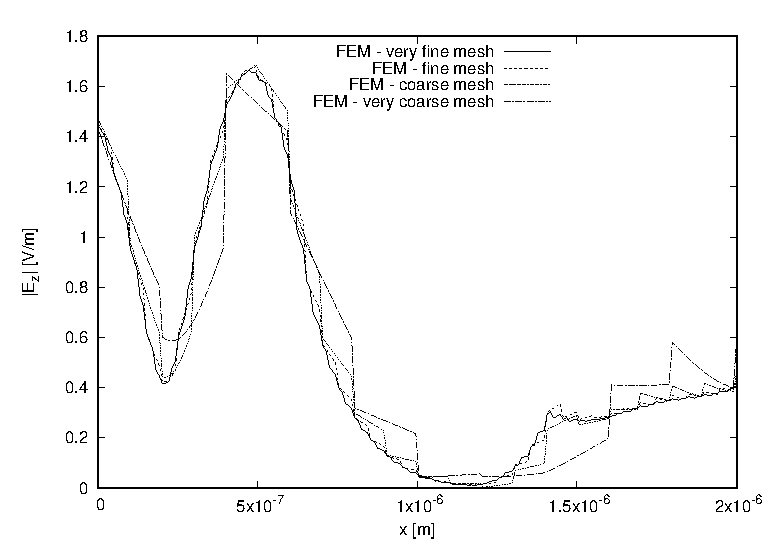
\includegraphics{figure_kraft_pendry_along_x_mag_ez_convergence.eps}
\caption{Convergence of the solution for problem involving medium of Kraft et al.
The magnitude of the $z$ component of the electric field is plotted 
along a line parallel to $x$ axis for four different meshes.}
\label{fi:kraft_pendry_convergence}
\end{figure}

The magnitudes and pahses of some for the components of the field 
along different axis directions are shown in 
Figures  \ref{fi:kraft_pendry_ez_vs_x} to \ref{fi:kraft_pendry_ez_vs_z}.
The solutions obtained for $\zeta_0 = -0.41$ are compared with that 
for the isotropic case ($\zeta_0 = 0$, $\varepsilon_r = -1 -j 0.4$, $\mu_r = 1$).
For example we can see in Figures \ref{fi:kraft_pendry_ez_vs_x} and \ref{fi:kraft_pendry_ez_vs_z}
that there are differences of 10 to 20 percent of the incident field in the 
magnitudes of the electric fields which are induced by the magneto electric coupling 
factor $\zeta_0$.
Likewise the phases of the fields are similarly affected by the bianisotropy of the medium.
These non negligible effects imply that the accuracy of the simulations requires the 
us to consider the bianisotropy of the medium.
Hence the reliability of the finite element silution in the presence of bianisotropy is important 
for getting good results for this kind of problems.
The appliaciton of our theory gives the conditions under which we can guarantee such reliability.


\begin{figure}[H]
\centering
\begin{subfigure}[b]{0.49\textwidth}
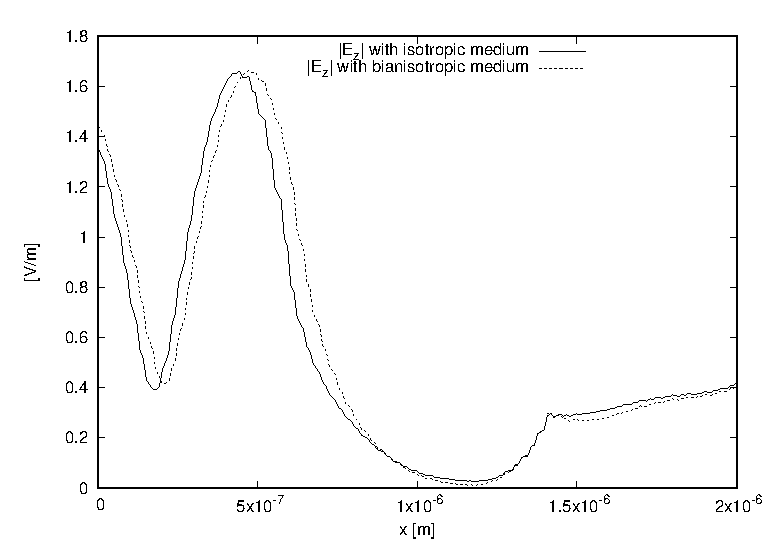
\includegraphics[width=\textwidth]{figure_kraft_pendry_along_x_mag_ez.eps}
\end{subfigure}
%
\begin{subfigure}[b]{0.49\textwidth}
\centering
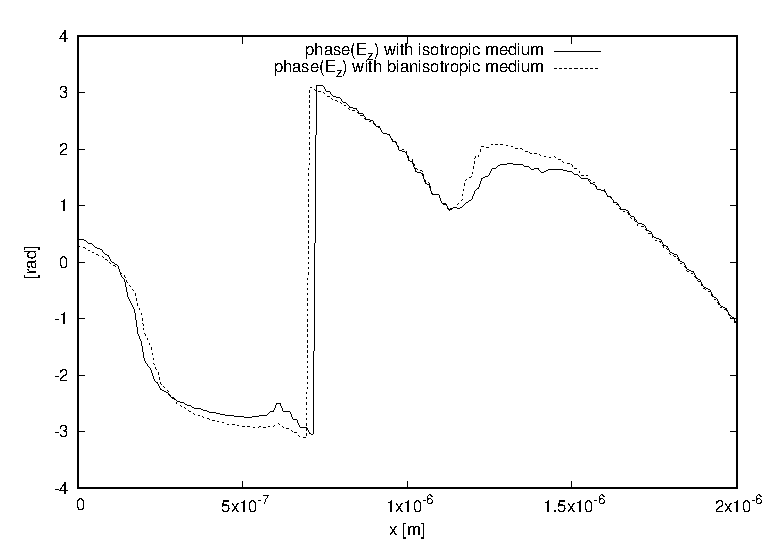
\includegraphics[width=\textwidth]{figure_kraft_pendry_along_x_phase_ez.eps}
\end{subfigure}
\caption{The magnitude and phase of the $z$ component of electric field along a line parallel to $x$ axis 
and passing though the center of gravity of the domain for problem involving medium of Kraft et al. 
The plots for bianisotropic case  using $\zeta_0 = -0.41$ is compared with 
the solution obtained in isotropic case using $\zeta_0 = 0$.}
\label{fi:kraft_pendry_ez_vs_x}
\end{figure}

\begin{figure}[H]
\centering
\begin{subfigure}[b]{0.49\textwidth}
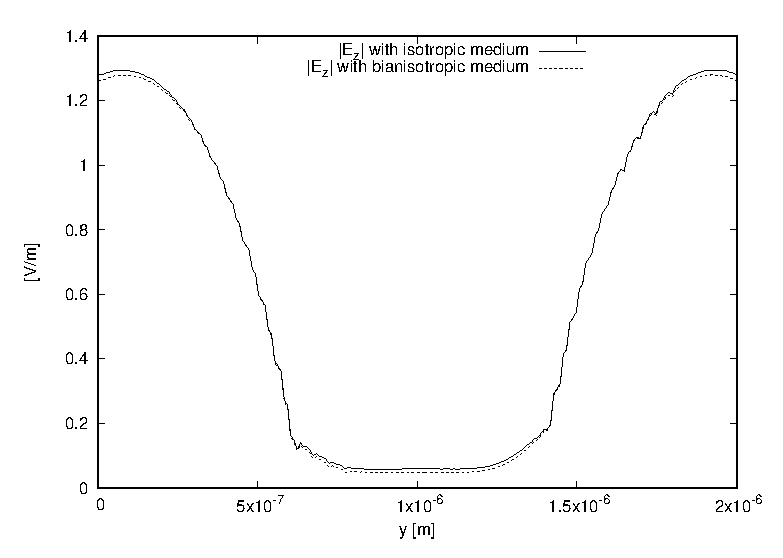
\includegraphics[width=\textwidth]{figure_kraft_pendry_along_y_mag_ez.eps}
\end{subfigure}
%
\begin{subfigure}[b]{0.49\textwidth}
\centering
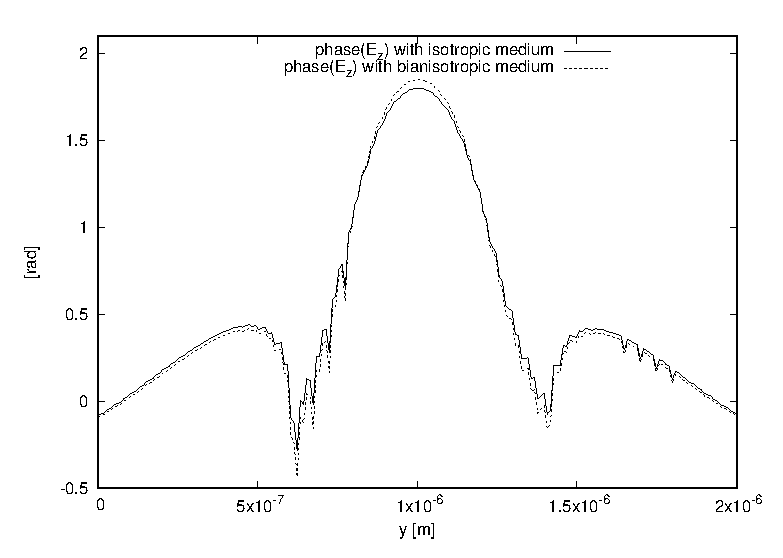
\includegraphics[width=\textwidth]{figure_kraft_pendry_along_y_phase_ez.eps}
\end{subfigure}
\caption{The magnitude and phase of the $z$ component of electric field along a line parallel to $y$ axis 
and passing though the center of gravity of the domain  for problem involving medium of Kraft et al. 
The plots for bianisotropic case using $\zeta_0 = -0.41$ is compared with 
the solution obtained in isotropic case using $\zeta_0 = 0$. }
\label{fi:kraft_pendry_ez_vs_y}
\end{figure}

\begin{figure}[H]
\centering
\begin{subfigure}[b]{0.49\textwidth}
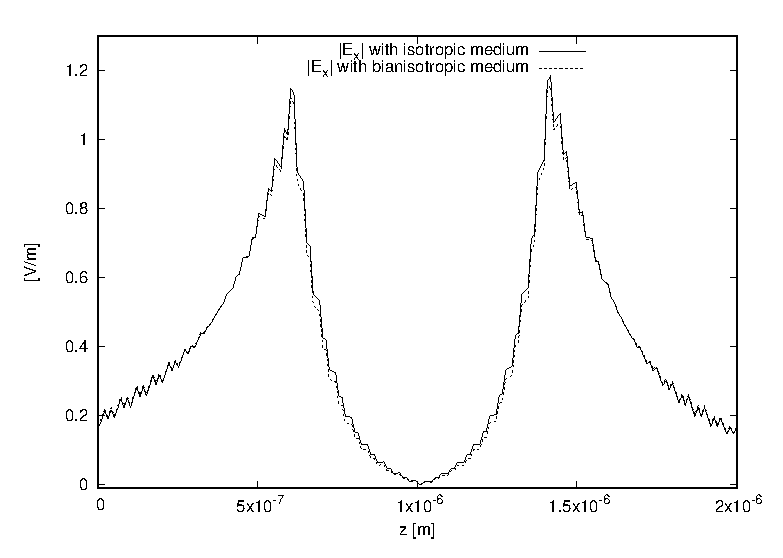
\includegraphics[width=\textwidth]{figure_kraft_pendry_along_z_mag_ex.eps}
\end{subfigure}
%
\begin{subfigure}[b]{0.49\textwidth}
\centering
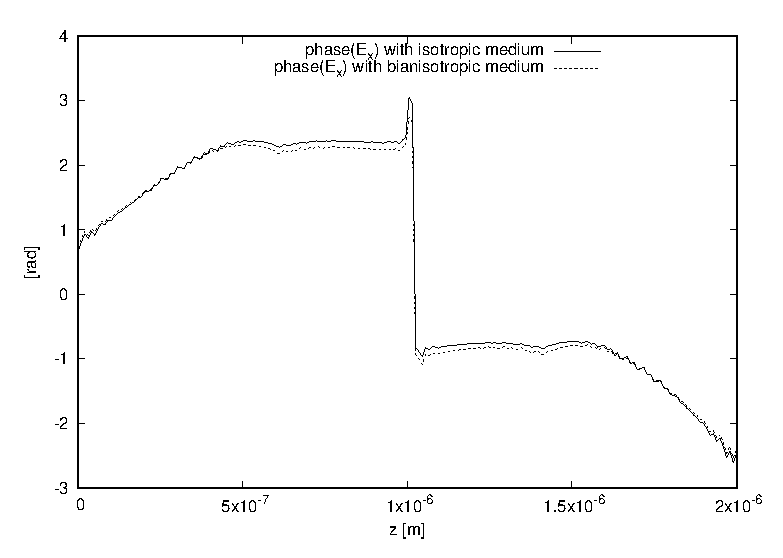
\includegraphics[width=\textwidth]{figure_kraft_pendry_along_z_phase_ex.eps}
\end{subfigure}
\caption{The magnitude and phase of the $x$ component of electric field along a line parallel to $z$ axis 
and passing though the center of gravity of the domain for problem involving medium of Kraft et al. 
The plots for bianisotropic case using $\zeta_0 = -0.41$ is compared with 
the solution obtained in isotropic case using $\zeta_0 = 0$.}
\label{fi:kraft_pendry_ex_vs_z}
\end{figure}

\begin{figure}[H]
\centering
\begin{subfigure}[b]{0.49\textwidth}
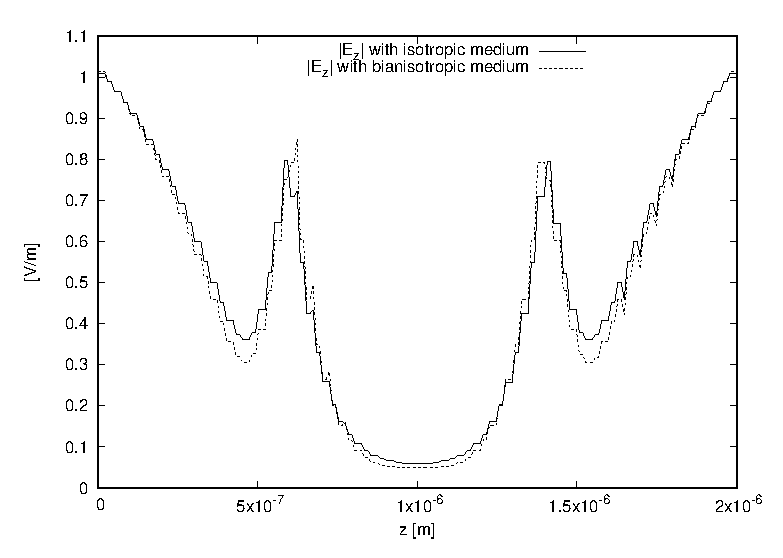
\includegraphics[width=\textwidth]{figure_kraft_pendry_along_z_mag_ez.eps}
\end{subfigure}
%
\begin{subfigure}[b]{0.49\textwidth}
\centering
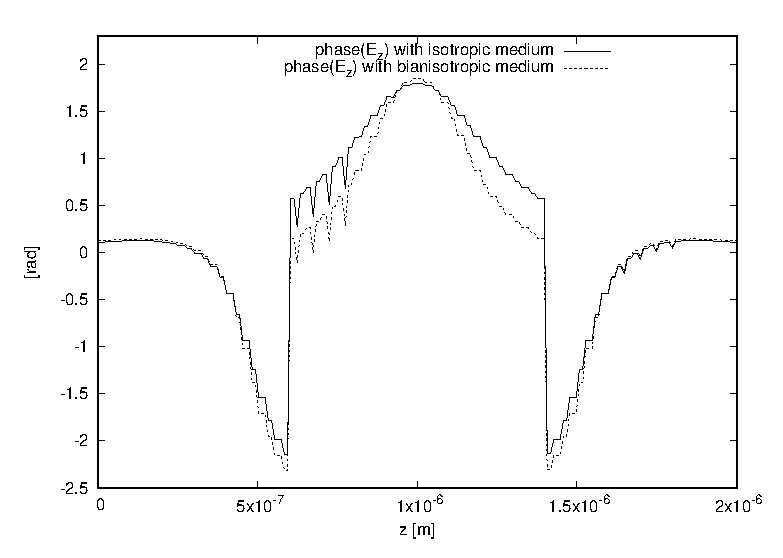
\includegraphics[width=\textwidth]{figure_kraft_pendry_along_z_phase_ez.eps}
\end{subfigure}
\caption{The magnitude and phase of the $z$ component of electric field along a line parallel to $z$ axis 
and passing though the center of gravity of the domain  for problem involving medium of Kraft et al. 
The plots for bianisotropic case using $\zeta_0 = -0.41$ is compared with 
the solution obtained in isotropic case using $\zeta_0 = 0$.}
\label{fi:kraft_pendry_ez_vs_z}
\end{figure}

\subsection{Chirowaveguides considered in \cite{wujaggard}}
In \cite{wujaggard}, the authors consider a waveguide partially filled with 
a chiral medial which is characterized by
\begin{equation}
\left\{
\begin{array}{ll}
{\bf D} = \varepsilon_0\varepsilon_r I_3 {\bf E} - j \xi_c I_3 {\bf B} \\
{\bf H} = -j\xi_c I_3 {\bf E} + \frac{1}{\mu_0\mu_r} I_3 {\bf B}.
\end{array}
\right.
\end{equation}

Here $\varepsilon_r$, $\mu_r$ and $\xi_c$ are strictly positive real quantities.


\subsection{Bianisotropic media considered in \cite{alottocodecasa}}
Another instance of a relevant bianisotropic media was considered in 
\cite{alottocodecasa}, where the authors consider a rectangular waveguide, 
half of which is empty and the other half is filled with a lossless bianisotropic material characterized by 

\begin{equation} \label{constitutive_alotto_P}
P = \varepsilon_0c_0 I_3,
\end{equation}

\begin{equation} \label{constitutive_alotto_Q}
Q = \frac{1}{\mu_0c_0} I_3, 
\end{equation}

\begin{equation} \label{constitutive_alotto_LM}
L = M = j\kappa_0 A ,
\end{equation}
where $A$ is the matrix given by

\begin{equation} \label{constitutive_alotto_LM}
A= 
\begin{bmatrix}
1 & 1 & 0 \\
1 & 1 & 0 \\
0 & 0 & 1 
\end{bmatrix},
\end{equation}
where $\kappa_0$ is a positive real number.

The hypotheses H5 and H6 are trivially valid with $C_{PS} = \varepsilon_0c_0$ and
$C_{QS} = \frac{1}{\mu_0c_0}$.
Further, $L^*L = M^*M =  \kappa_0^2A^2$ whose eigenvalues are 0, $\kappa_0^2$ and $4\kappa_0^2$.
Therefore by equations \eqref{equation_for_CL} and \eqref{equation_for_CM} we get $C_L = C_M = 2\kappa_0$.
The condition in hypothesis H7 then becomes 
$C_{QS} - \frac{C_L C_M}{C_{PS}} = \frac{1}{\mu_0c_0} - \frac{4\kappa_0^2}{\varepsilon_0c_0} > 0$, 
which gives the following limit on $\kappa_0$.

\begin{equation} \label{eq:uniqueness_cond_alotto_codecasa}
\kappa_0 < \frac{1}{2}\sqrt{\frac{\varepsilon_0}{\mu_0}} = 1.327 \, 10^{-3}   \text{ mho }
\end{equation}

The hypotheses H1 to H4 can be studied using the alternative form of constitutive relations
which is characterized by the following matrices \cite{noiregolarita}.

\begin{equation}
\kappa =\frac{1}{\varepsilon_0}I_3
\end{equation}

\begin{equation}
\nu =\frac{1}{\mu_0}I_3 + \frac{\kappa_0^2}{\varepsilon_0}A^2
\end{equation}

\begin{equation}
\chi = -\gamma = \frac{-j\kappa_0}{\varepsilon_0}A
\end{equation}

The determinants of $\kappa$ and $\nu$ can be readily calculated and by using equations
\eqref{equation_for_C_kd} and \eqref{equation_for_C_nud} we get $C_{\kappa,d}$ and $C_{\nu,d}$.

\begin{equation}
C_{\kappa,d} = \frac{1}{\varepsilon_0^3}
\end{equation}

\begin{equation}
C_{\nu,d} =  \frac{(\varepsilon_0+\mu_0\kappa_0^2)(\varepsilon_0+4\mu_0\kappa_0^2)}{\mu_0^3\varepsilon_0^2}
\end{equation}

$C_{\kappa,s}$ and $C_{\nu,s}$ can be directly obtained from their definitions.

\begin{equation}
C_{\kappa,s} = \frac{2}{\varepsilon_0}
\end{equation}

\begin{equation}
C_{\nu,s} = \frac{2\varepsilon_0 + 8\mu_0\kappa_0^2}{\mu_0\varepsilon_0}
\end{equation}

By simple application of the definition
\begin{equation}
C_{\kappa,r} = \varepsilon_0 ,
\end{equation}
and by equation \eqref{equation_for_C_nur}  $C_{\nu,r}$ evaluates to the reciprocal of the largest 
eigenvalue of the real matrix $\nu$ which is given by
\begin{equation}
C_{\nu,r} =  \frac{\mu_0\varepsilon_0}{\varepsilon_0 + 4 \mu_0\kappa_0^2}.
\end{equation}

The equations  \eqref{equation_for_C_chis} and \eqref{equation_for_C_gammas} give 

\begin{equation}
C_{\chi,s} = C_{\gamma,s}= = \frac{4\kappa_0}{\varepsilon_0}.
\end{equation}

The existence of the above constants verifies H1 -H3 and we can use them to 
calculate $K_u$ to verify H4.
It can be verified that $K_u$ is less than one when $\kappa_0 \leq 2.72 \, 10^{-4}$ mho,
which is stricter than the limit obtained from equation \eqref{eq:uniqueness_cond_alotto_codecasa}.

Finally let us give some numerical solutions for this problem, which can be used as benchmarks for other 
approaches.
The cross section of the waveguide is such that it is 2 cm along the x axis and  1 cm along the y axis, and 
the length of the waveguide is 2 cm, half of which is filled with the bianisotropic medium  characterized by 
$\kappa_0 = 2.7 \, 10^{-3}$.
The origin is taken on the corner of the open face of the waveguide on the empty side.
$TE_{10}$ mode is excited in the waveguide with source of amplitude 1 $V/m$ and frequency of 12 GHz.

First order edge element based Galerkin finite element method is used to obtain the solution.
The meshing is carried out by dividing the domain into identical cubes each of which are then 
subdivided into six tetrahedra.
Convergence is ensured by evaluating the solutions on three meshes, 
termed as ``coarse'', ``fine'' and ``very fine'' characterized, respectively, by cubes of sides 1 mm, 
0.5 mm and 0.33 mm.
The coarse mesh had 4852 nodes, 24000 elements and 3200 boundary faces.
The fine mesh is composed of 35301 nodes, 192000 elements and 12800 boundary faces.
The very fine mesh has 115351 nodes, 648000 elements and 28800 boundary faces.
Figure \ref{fi:alotto_codecasa_convergence} shows the results obtained on the three 
meshes for the x component of the electric field along the y axis and confirms the 
stability of the solutions.

\begin{figure}
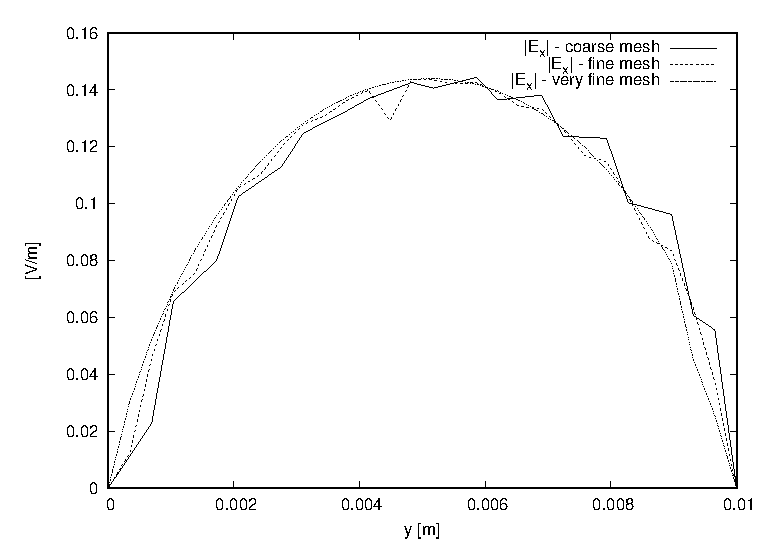
\includegraphics{figure_convergence_alotto_codecasa_along_y_mag_ex.eps}
\caption{Convergence of the solution for problem involving medium in \cite{alottocodecasa}.
The magnitude of the $x$ component of the electric field is plotted
along a line parallel to $y$ axis for four different meshes.}
\label{fi:alotto_codecasa_convergence}
\end{figure}

We provide the magnitudes and phases of the components of the electric field obtained from the 
simulation in Figures \ref{fi:alotto_codecasa_xaxis_ex} to \ref{fi:alotto_codecasa_zaxis_ez}.
It can be observed that the bianisotropic effects are non negligible and the largest effects 
are on the x component of the field.
The bianisotropy causes a difference in magnitude of up to 14 percent of the incident 
field, as can be seen,  for example, from Figure  \ref{fi:alotto_codecasa_xaxis_ex}, 
\ref{fi:alotto_codecasa_yaxis_ex} or  \ref{fi:alotto_codecasa_zaxis_ex}.
Since the theory guarantees the reliability of these results, it can be used as benchmark for 
other solvers and approaches.


\begin{figure}
\centering
\begin{subfigure}[b]{0.49\textwidth}
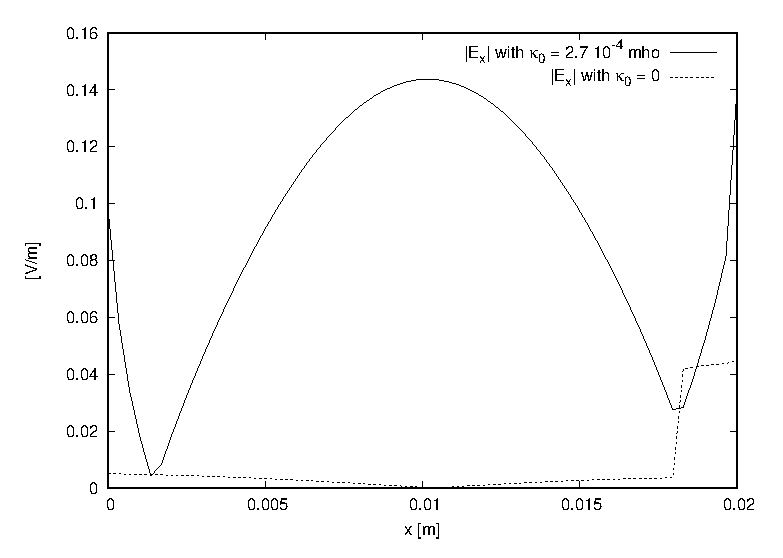
\includegraphics[width=\textwidth]{figure_alotto_codecasa_along_x_mag_ex.eps}
\end{subfigure}
%
\begin{subfigure}[b]{0.49\textwidth}
\centering
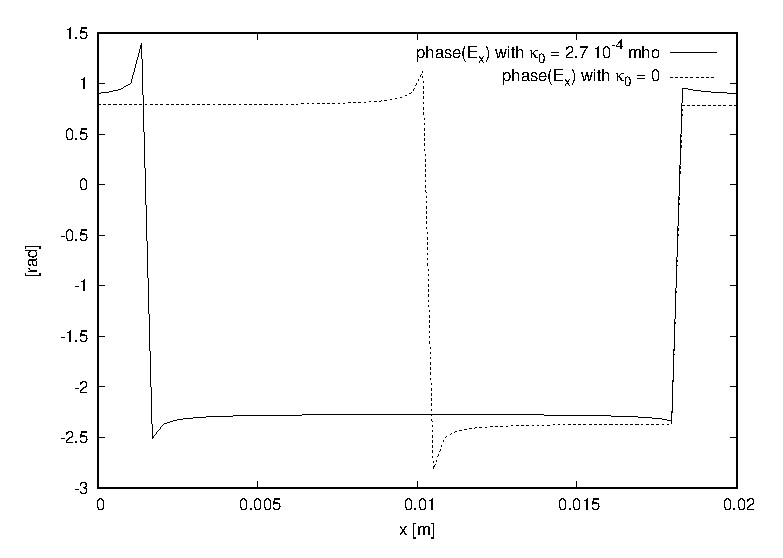
\includegraphics[width=\textwidth]{figure_alotto_codecasa_along_x_phase_ex.eps}
\end{subfigure}
\caption{The magnitude and phase of the $x$ component of electric field along a line parallel to $x$ axis 
and passing though the center of gravity of the domain for problem involving 
medium in \cite{alottocodecasa}. 
The plot for bianisotropic case  using $\kappa_0 = 2.7\,10^{-4}$ mho is compared with 
the solution obtained in isotropic case using $\kappa_0 = 0$.}
\label{fi:alotto_codecasa_xaxis_ex}
\end{figure}

\begin{figure}
\centering
\begin{subfigure}[b]{0.49\textwidth}
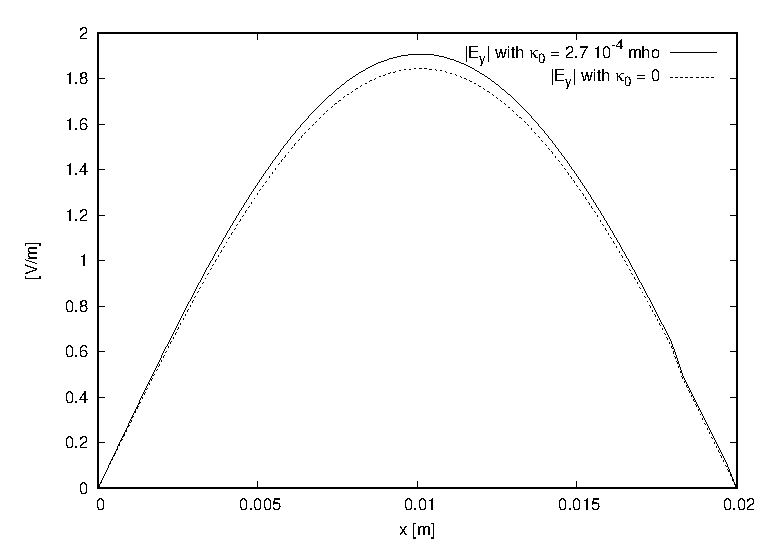
\includegraphics[width=\textwidth]{figure_alotto_codecasa_along_x_mag_ey.eps}
\end{subfigure}
%
\begin{subfigure}[b]{0.49\textwidth}
\centering
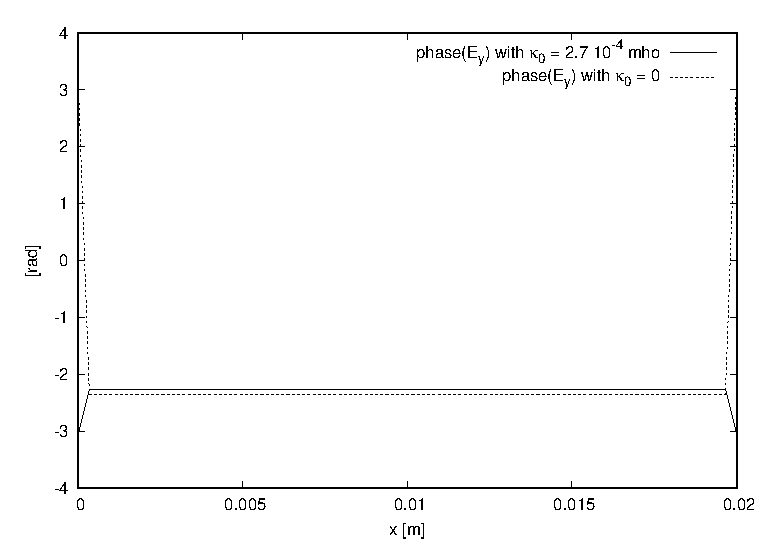
\includegraphics[width=\textwidth]{figure_alotto_codecasa_along_x_phase_ey.eps}
\end{subfigure}
\caption{The magnitude and phase of the $y$ component of electric field along a line parallel to $x$ axis 
and passing though the center of gravity of the domain for problem involving 
medium in \cite{alottocodecasa}. 
The plot for bianisotropic case  using $\kappa_0 = 2.7\,10^{-4}$ mho is compared with 
the solution obtained in isotropic case using $\kappa_0 = 0$.}
\label{fi:alotto_codecasa_xaxis_ey}
\end{figure}

\begin{figure}
\centering
\begin{subfigure}[b]{0.49\textwidth}
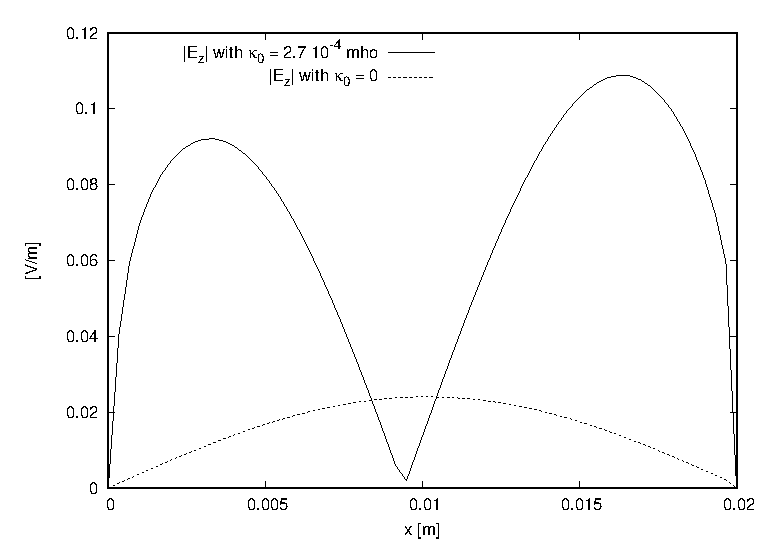
\includegraphics[width=\textwidth]{figure_alotto_codecasa_along_x_mag_ez.eps}
\end{subfigure}
%
\begin{subfigure}[b]{0.49\textwidth}
\centering
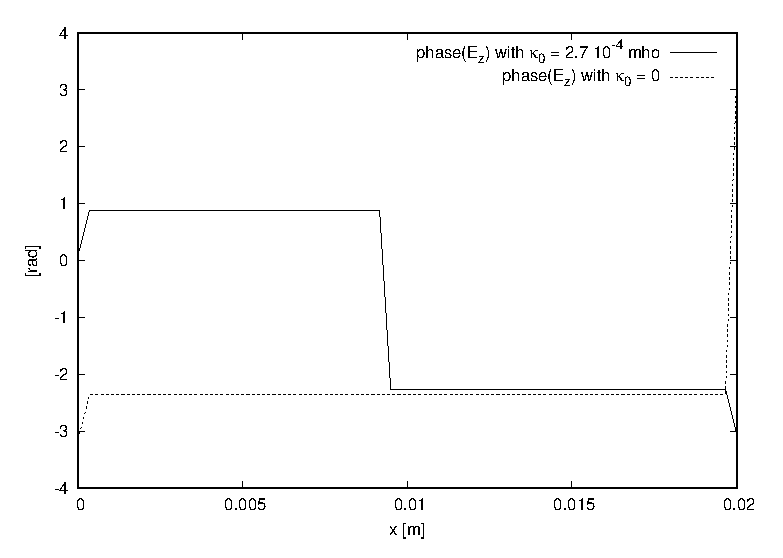
\includegraphics[width=\textwidth]{figure_alotto_codecasa_along_x_phase_ez.eps}
\end{subfigure}
\caption{The magnitude and phase of the $z$ component of electric field along a line parallel to $x$ axis 
and passing though the center of gravity of the domain for problem involving 
medium in \cite{alottocodecasa}. 
The plot for bianisotropic case  using $\kappa_0 = 2.7\,10^{-4}$ mho is compared with 
the solution obtained in isotropic case using $\kappa_0 = 0$.}
\label{fi:alotto_codecasa_xaxis_ez}
\end{figure}

\begin{figure}
\centering
\begin{subfigure}[b]{0.49\textwidth}
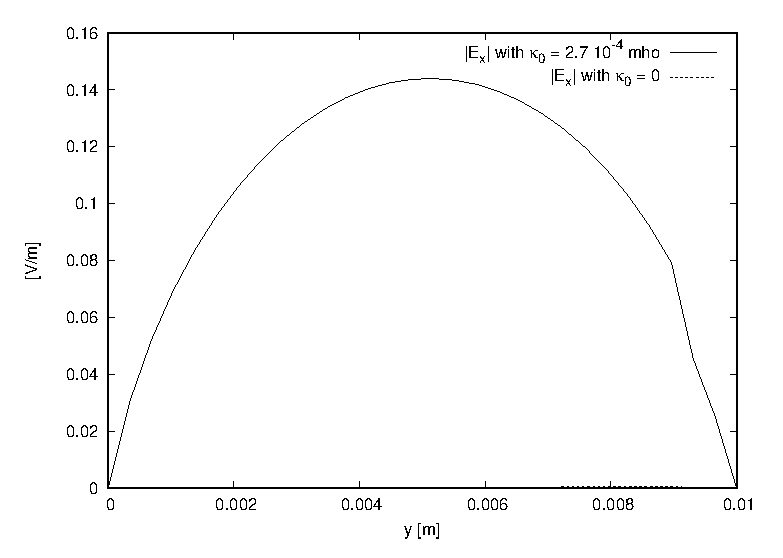
\includegraphics[width=\textwidth]{figure_alotto_codecasa_along_y_mag_ex.eps}
\end{subfigure}
%
\begin{subfigure}[b]{0.49\textwidth}
\centering
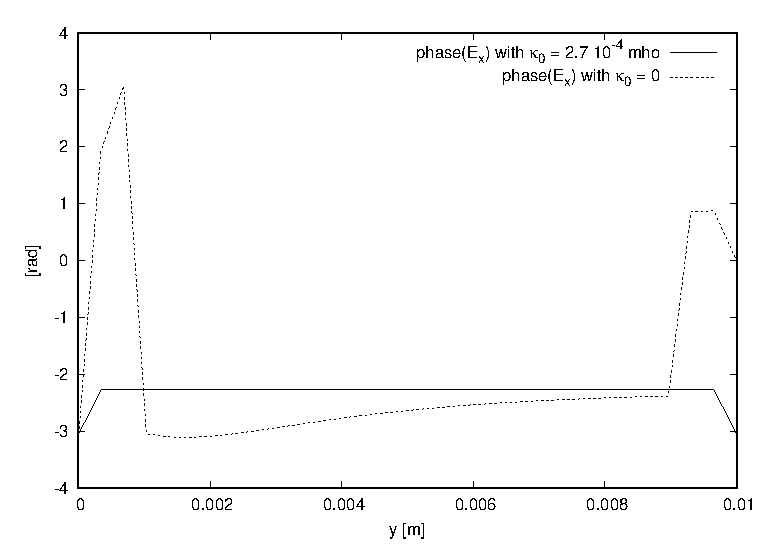
\includegraphics[width=\textwidth]{figure_alotto_codecasa_along_y_phase_ex.eps}
\end{subfigure}
\caption{The magnitude and phase of the $x$ component of electric field along a line parallel to $y$ axis 
and passing though the center of gravity of the domain for problem involving 
medium in \cite{alottocodecasa}. 
The plot for bianisotropic case  using $\kappa_0 = 2.7\,10^{-4}$ mho is compared with 
the solution obtained in isotropic case using $\kappa_0 = 0$.}
\label{fi:alotto_codecasa_yaxis_ex}
\end{figure}

\begin{figure}
\centering
\begin{subfigure}[b]{0.49\textwidth}
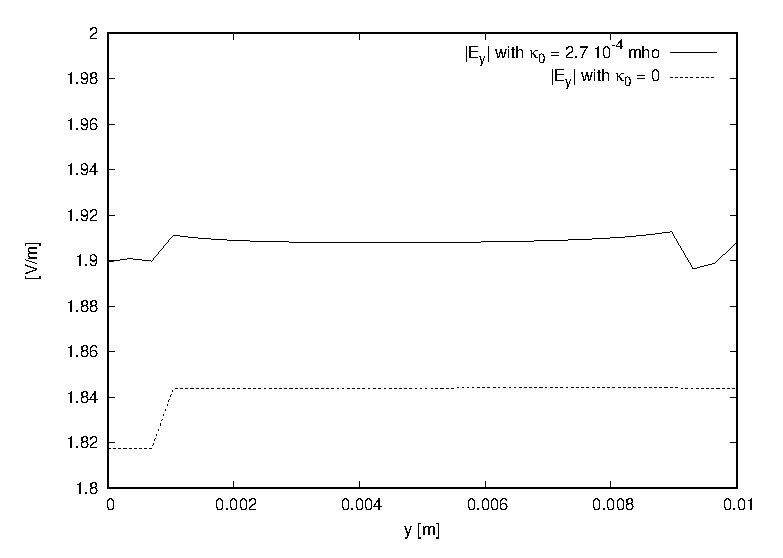
\includegraphics[width=\textwidth]{figure_alotto_codecasa_along_y_mag_ey.eps}
\end{subfigure}
%
\begin{subfigure}[b]{0.49\textwidth}
\centering
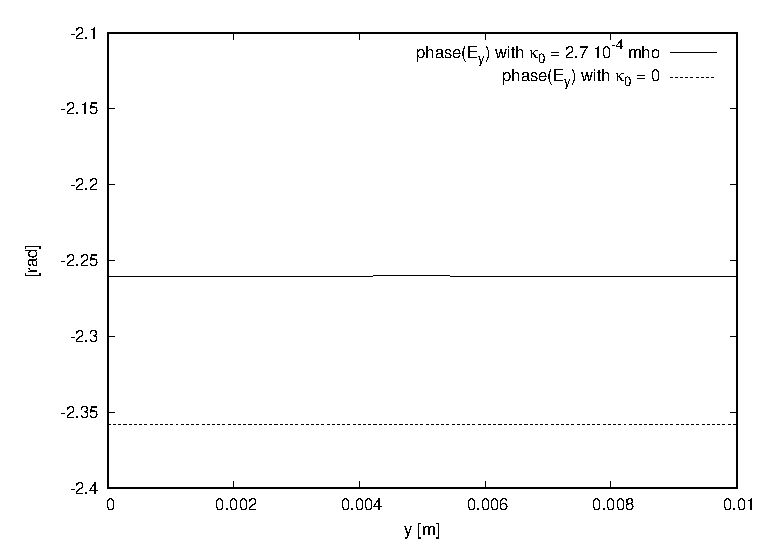
\includegraphics[width=\textwidth]{figure_alotto_codecasa_along_y_phase_ey.eps}
\end{subfigure}
\caption{The magnitude and phase of the $y$ component of electric field along a line parallel to $y$ axis 
and passing though the center of gravity of the domain for problem involving 
medium in \cite{alottocodecasa}. 
The plot for bianisotropic case  using $\kappa_0 = 2.7\,10^{-4}$ mho is compared with 
the solution obtained in isotropic case using $\kappa_0 = 0$.}
\label{fi:alotto_codecasa_yaxis_ey}
\end{figure}

\begin{figure}
\centering
\begin{subfigure}[b]{0.49\textwidth}
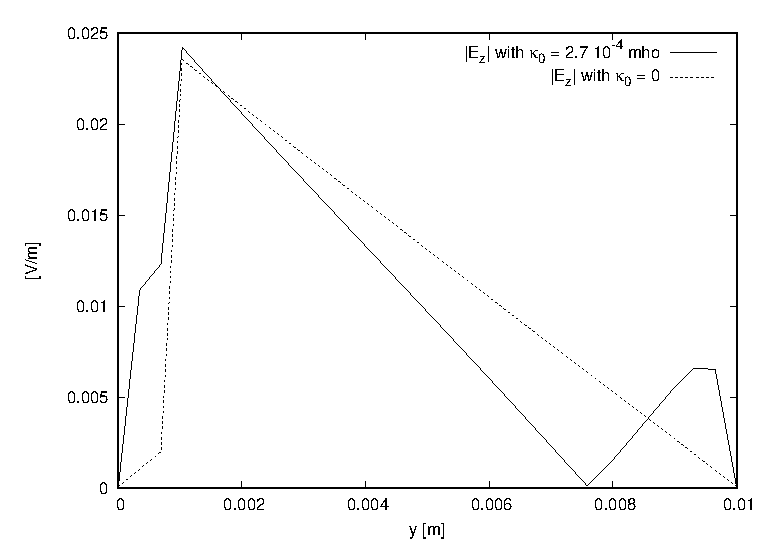
\includegraphics[width=\textwidth]{figure_alotto_codecasa_along_y_mag_ez.eps}
\end{subfigure}
%
\begin{subfigure}[b]{0.49\textwidth}
\centering
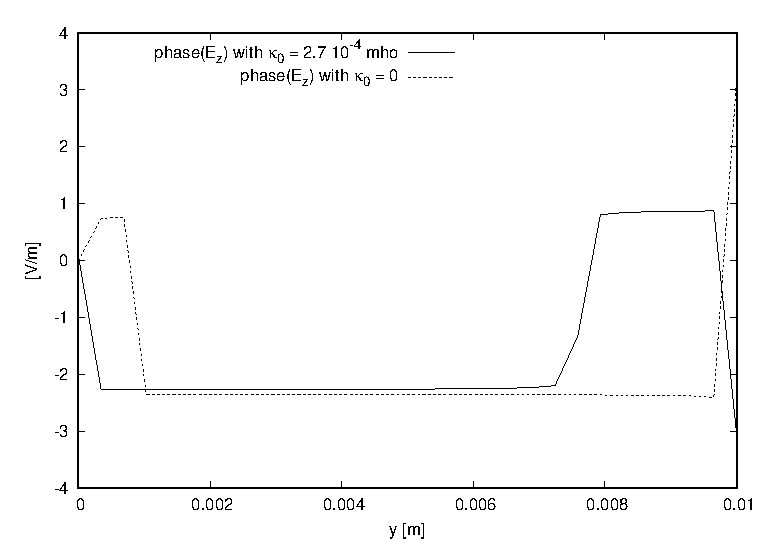
\includegraphics[width=\textwidth]{figure_alotto_codecasa_along_y_phase_ez.eps}
\end{subfigure}
\caption{The magnitude and phase of the $z$ component of electric field along a line parallel to $y$ axis 
and passing though the center of gravity of the domain for problem involving 
medium in \cite{alottocodecasa}. 
The plot for bianisotropic case  using $\kappa_0 = 2.7\,10^{-4}$ mho is compared with 
the solution obtained in isotropic case using $\kappa_0 = 0$.}
\label{fi:alotto_codecasa_yaxis_ez}
\end{figure}

\begin{figure}
\centering
\begin{subfigure}[b]{0.49\textwidth}
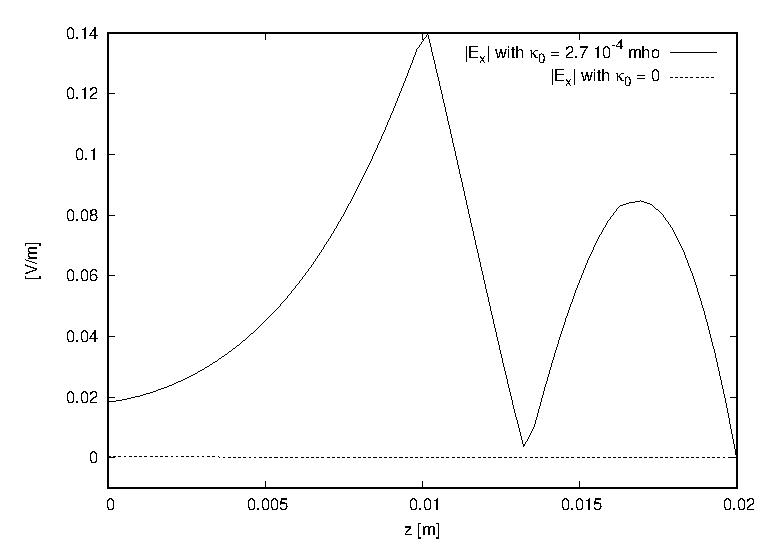
\includegraphics[width=\textwidth]{figure_alotto_codecasa_along_z_mag_ex.eps}
\end{subfigure}
%
\begin{subfigure}[b]{0.49\textwidth}
\centering
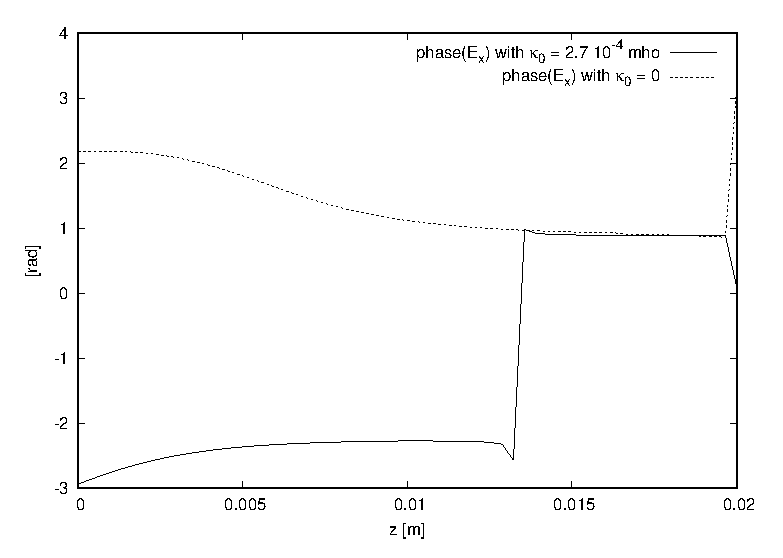
\includegraphics[width=\textwidth]{figure_alotto_codecasa_along_z_phase_ex.eps}
\end{subfigure}
\caption{The magnitude and phase of the $x$ component of electric field along a line parallel to $z$ axis 
and passing though the center of gravity of the domain for problem involving 
medium in \cite{alottocodecasa}. 
The plot for bianisotropic case  using $\kappa_0 = 2.7\,10^{-4}$ mho is compared with 
the solution obtained in isotropic case using $\kappa_0 = 0$.}
\label{fi:alotto_codecasa_zaxis_ex}
\end{figure}

\begin{figure}
\centering
\begin{subfigure}[b]{0.49\textwidth}
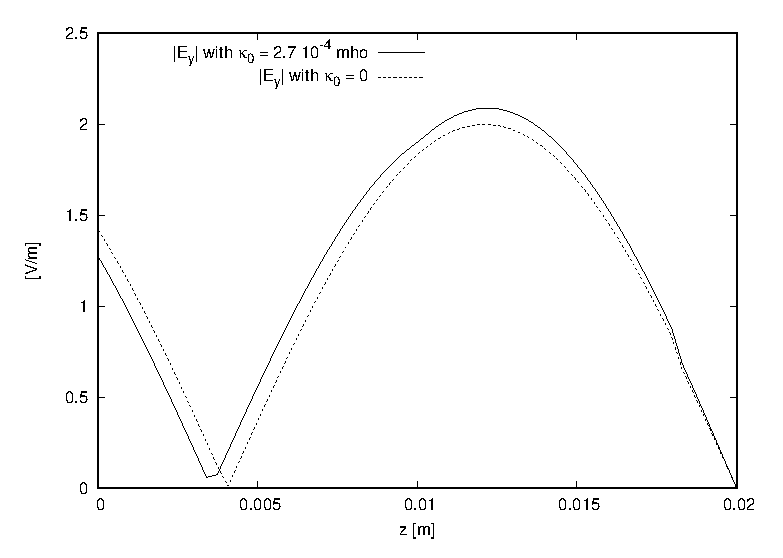
\includegraphics[width=\textwidth]{figure_alotto_codecasa_along_z_mag_ey.eps}
\end{subfigure}
%
\begin{subfigure}[b]{0.49\textwidth}
\centering
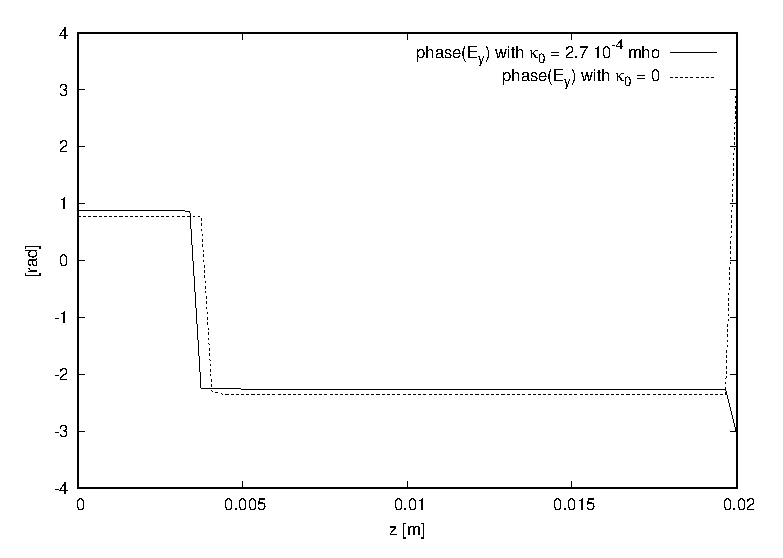
\includegraphics[width=\textwidth]{figure_alotto_codecasa_along_z_phase_ey.eps}
\end{subfigure}
\caption{The magnitude and phase of the $y$ component of electric field along a line parallel to $z$ axis 
and passing though the center of gravity of the domain for problem involving 
medium in \cite{alottocodecasa}. 
The plot for bianisotropic case  using $\kappa_0 = 2.7\,10^{-4}$ mho is compared with 
the solution obtained in isotropic case using $\kappa_0 = 0$.}
\label{fi:alotto_codecasa_zaxis_ey}
\end{figure}

\begin{figure}
\centering
\begin{subfigure}[b]{0.49\textwidth}
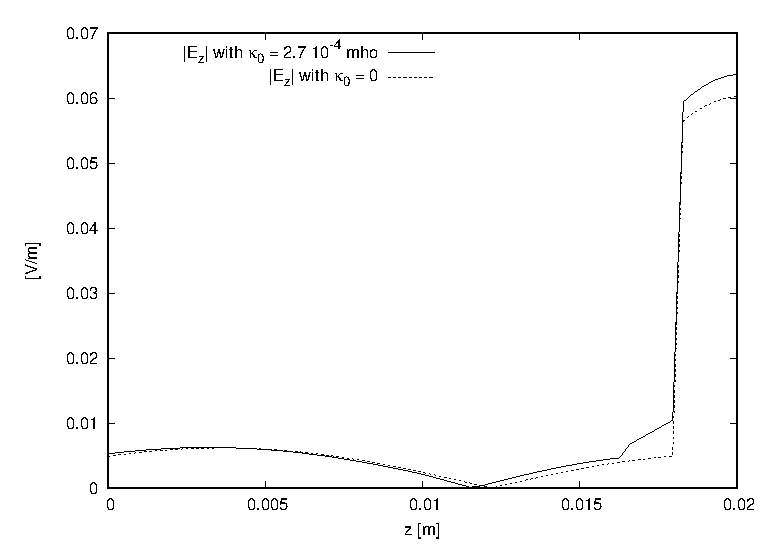
\includegraphics[width=\textwidth]{figure_alotto_codecasa_along_z_mag_ez.eps}
\end{subfigure}
%
\begin{subfigure}[b]{0.49\textwidth}
\centering
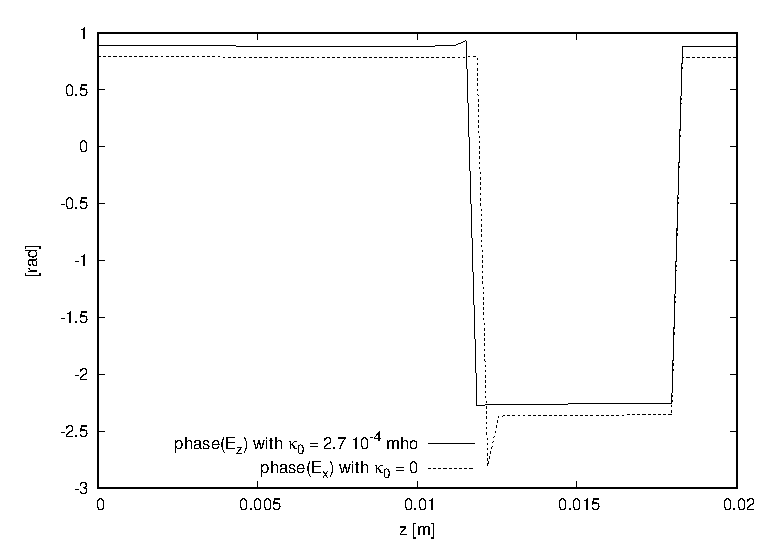
\includegraphics[width=\textwidth]{figure_alotto_codecasa_along_z_phase_ez.eps}
\end{subfigure}
\caption{The magnitude and phase of the $z$ component of electric field along a line parallel to $z$ axis 
and passing though the center of gravity of the domain for problem involving 
medium in \cite{alottocodecasa}. 
The plot for bianisotropic case  using $\kappa_0 = 2.7\,10^{-4}$ mho is compared with 
the solution obtained in isotropic case using $\kappa_0 = 0$.}
\label{fi:alotto_codecasa_zaxis_ez}
\end{figure}


\section{Conclusions}


\bibliographystyle{IEEEtran}
\bibliography{myreferences}
\end{document}
